\DiaryEntry{Groups - Subgroups}{2016-03-29}{Algebra}

Let G be a group and we select a number of group elements. Define S to
be the subset of G containing all possible group operations between
these elements and their inverses, in any order, and with repetition
allowed. Then S is a subgroup of G.

Select three elements and call them a,b, and c. Then e.g.
\(ab, abc, a^2bc, a^{-1}b a c^2 \in S\). We say that the subgroup S has
generators \(a, b, c\).

In the sepcial case of selecting one element, we obtain cyclic groups
which are denoted by \(G = \langle a \rangle\) where a is the
corresponding generator. The combination of operations with \(a\) and
\(a^{-1}\) becomes simple, as e.g. \(a a^{-1}\) cancel each other out.
Therefore, the cyclic group \(G = \langle a \rangle\) contains

\[
\cdots a^{-2}, a^{-1}, 1, a, a^2 \cdots
\]

\subsection{Cayley Diagrams}\label{cayley-diagrams}

Every finite group can be represented by a Cayley diagram: there is one
point for every element in the group. The arrows represent the result of
multiplying by a generator. In case there are several generators, the
arrows need to encode the information which operator is used (e.g.~by
chossing different colors).

That is, a Cayley diagram shows the effect of multiplying two elements
\(a\) and \(b\) together: select \(a\) as starting point and follow the
arrow corresponding to operation \(b\) in order to reach the point
\(a \star b\).

The Figure below shows an example of a Cayley diagram. Red arrows
correspond to multiplication with \(a\), blue arrows indicate
multiplication with \(b\). If we start at \(1\) and follow the red upper
lines, we see that we reach \(a\) and \(a^2\) by subsequently
multiplying \(1\) with \(a\). If we start at \(a\) and multiply with
\(b\), we reach the point \(ab\); conversely, if we start at \(b\) and
multiply with \(a\), we reach \(ba\). In case the group operation is
commutative, the points \(ab\) and \(ba\) become the same.

\begin{figure}[H]
\centering
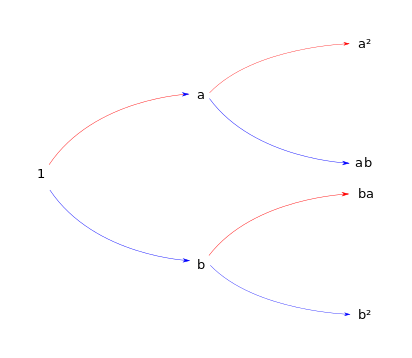
\includegraphics{images/groups_06_1.png}
\caption{Page1}
\end{figure}
